\chapter{Resultate}

\section{Harvesterschaltung}

\subsection{Leistungskurve Harvester}

Essentiell ist es zu wissen, wie viel Energie mit der Harvesterschaltung gewonnen werden kann. Dafür wurde die Leistungskurve des Harvesters aufgenommen. Die maximale Leistung hängt von der Geschwindigkeit ab, desto höher die Geschwindigkeit desto grösser die maximale Leistung. Bei einer Geschwindigkeit von 10 km/h kann bereits eine Leistung von ca. 25 $\mu$W generiert werden.

\begin{figure}[ht]
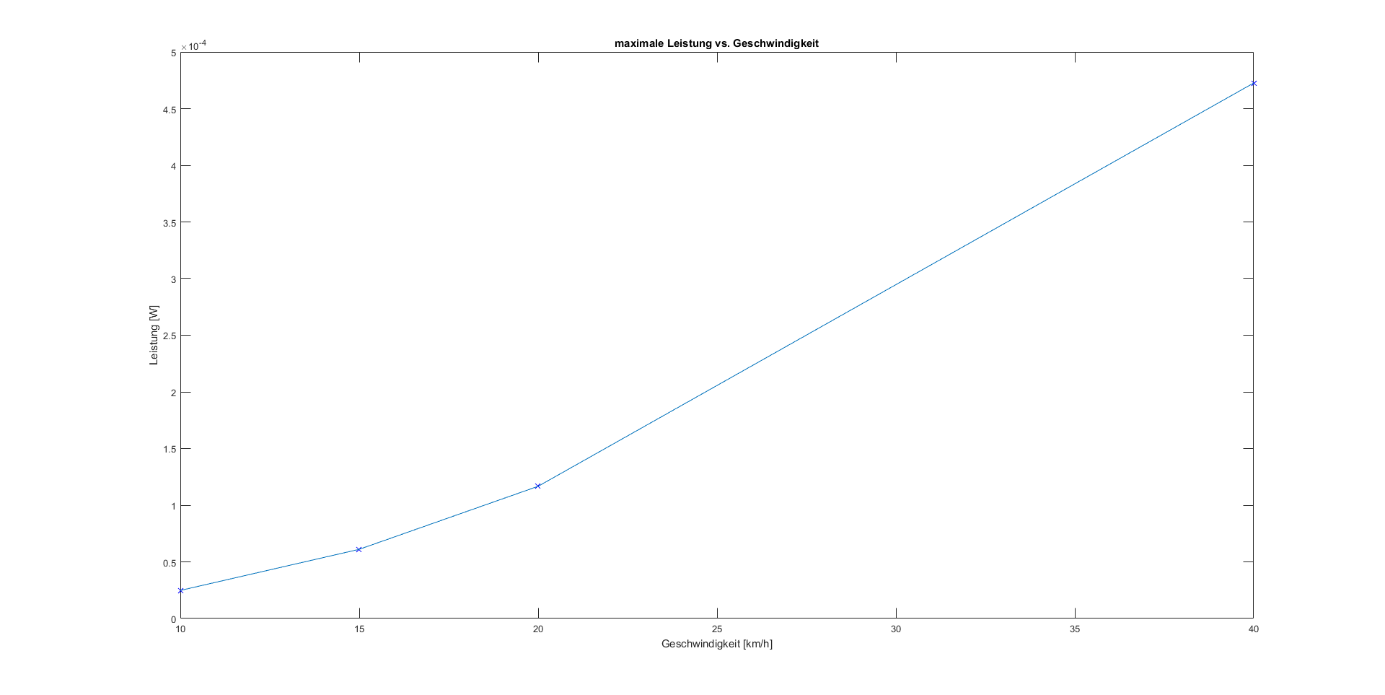
\includegraphics[width=0.5\textwidth]{4Resultate/imag/ResultatLeistungGeschwindigkeit.png} 
\caption{Maximale Leistung vs. Geschwindigkeit}
\end{figure}

Wichtig ist auch wo der MPP liegt, da der EM-Chip versucht am Eingang eine Leistungsanpassung zu erlangen, damit die maximale Leistung von der Harvesterquelle bezogen werden kann. Dieser MPP ist jedoch je nach Geschwindigkeit an einer anderen Stelle, d.h. der MPP hängt von der Geschwindigkeit ab und das Verhältnis von Open Loop Spannung zu der Spannung des MPP ändert sich. Dieses Verhältnis kann beim EM-Chip eingestellt werden, jedoch ist der wandernde MPP ein Problem, da ein fixes Verhältnis eingestellt werden muss.

\begin{figure}[ht]
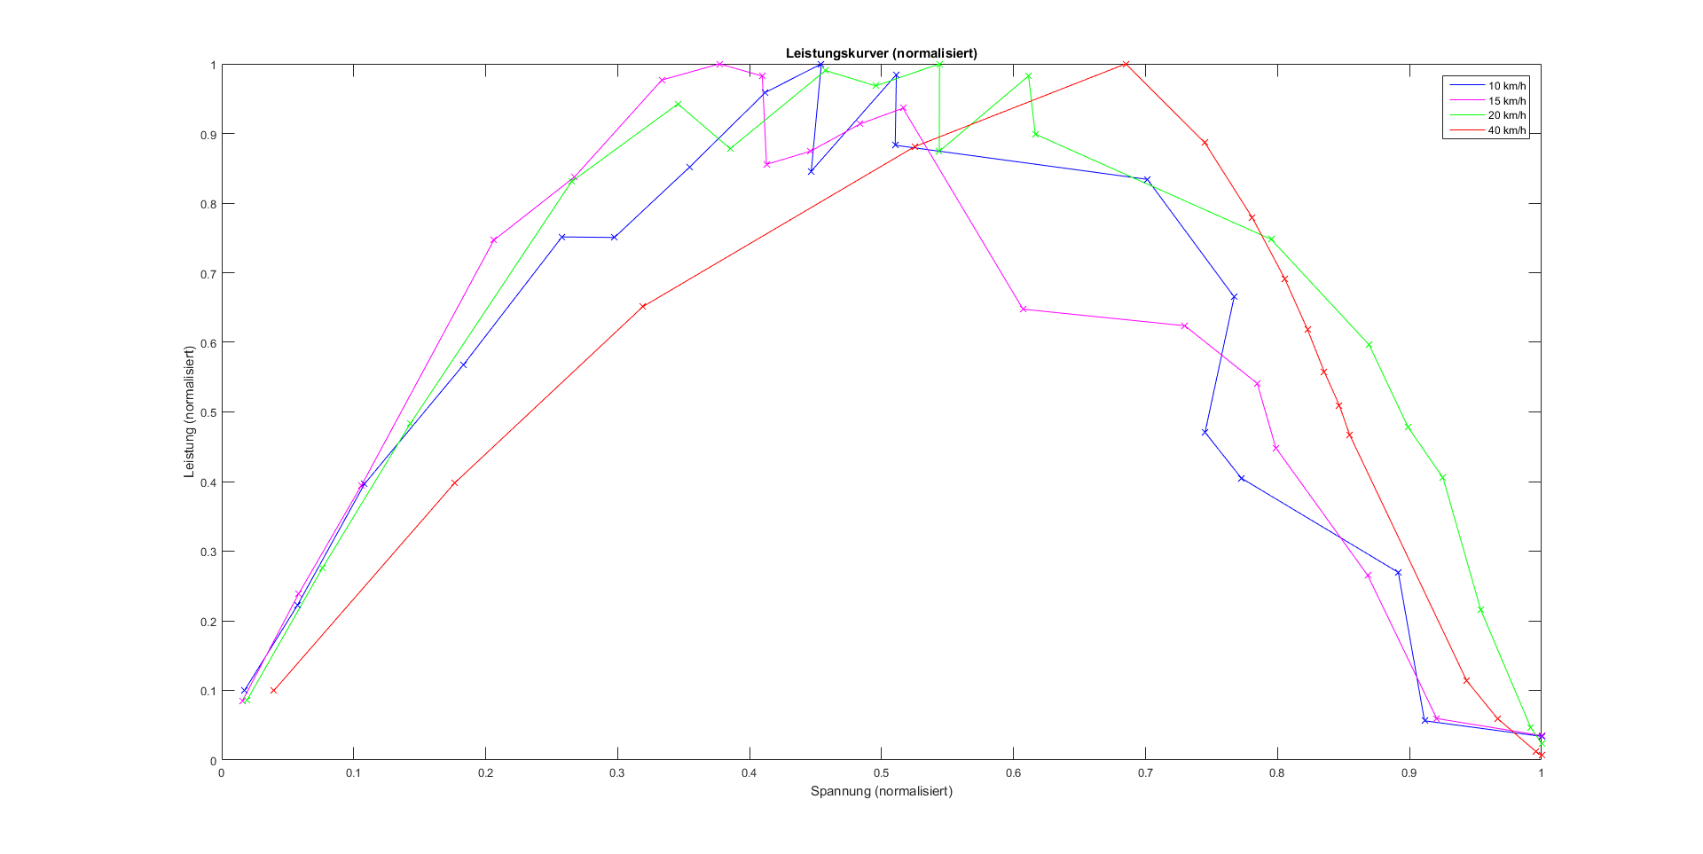
\includegraphics[width=0.5\textwidth]{4Resultate/imag/MPPHarvester.png} 
\caption{Leistungskurve (normalisiert) }
\end{figure}


\subsection{Harvesterausgang}

Die Spannung am Harvesterausgang bzw. am Eingang des EM-Chip ist sehr kritisch, da von dieser Spannung die gewonnene Energie abhängt. Das bedeutet, dass eine schwankende oder nicht ordentlich geregelte Spannung ein Problem für die Energiegewinnung darstellt. 
Der EM-Chip regelt den Eingang anhand der Messung der Open Loop Spannung auf ein voreingestelltes Level, was durch die Einstellung des MPPT-Ratio beeinflusst werden kann. Optimalerweise handelt es sich bei der Spannung am Eingang des EM-Chips um eine Gleichspannung, jedoch wird mit der verwendeten Harvesterquelle keine konstante Gleichspannung generiert, sondern eine Gleichspannung mit einem Rippel. Die Rippelspannung macht die Regelung sehr instabil und liefert teilweise falsche Open Loop Messresultate. 
Entscheidend ist die Kapazität vom Kondensator C2 am Ausgang des Harvesters. Eine hohe Kapazität des Kondensators resultiert in einer geringen Rippelspannung, jedoch nicht korrekten Open Loop Messungen, da sich der Kondensator langsam auflädt. Eine geringe Kapazität des Kondensators resultiert in einer grossen Rippelspannung, jedoch in besseren Open Loop Messungen, da sich der Kondensator schnell auflädt. Somit muss abgeschätzt werden, wie man den Kondensator dimensioniert.
Eine Kapazität von 100 $\mu$F ist gemäss den Messresultaten des Messprotokolls «hier Link einfügen» ein guter Kompromiss. Die Open Loop Messungen des EM-Chips sind sicherlich nicht richtig, jedoch ist die geregelte Spannung VCC relativ stabil. Ebenfalls liegt die geregelte Spannung über 0.3 V, was die minimale Spannung zur Energiegewinnung ist. Natürlich ist die Spannung am Eingang des EM-Chips keine konstante Gleichspannung, jedoch fluktuiert die Spannung nicht zu stark, dass die Regelung nicht funktionieren würde.

\begin{figure}[ht]
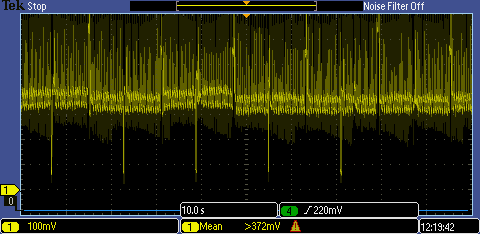
\includegraphics[width=0.5\textwidth]{4Resultate/imag/SpannungVCC.png} 
\caption{Spannung VCC bei 15 km/h }
\end{figure}

\subsection{Wirkungsgrad der Schaltung}

In den Messprotokollen (xxxx) auf der CD sind diverse Energiemessungen dokumentiert. Die Abbildung \ref{zsmEnergyGewinn} gibt einen Überblick, an welcher Stelle wie viel Energie vorhanden ist, bzw. zwischen welchen zwei Stellen wie viel Energie verloren ging.

\begin{figure}\label{zsmEnergyGewinn}
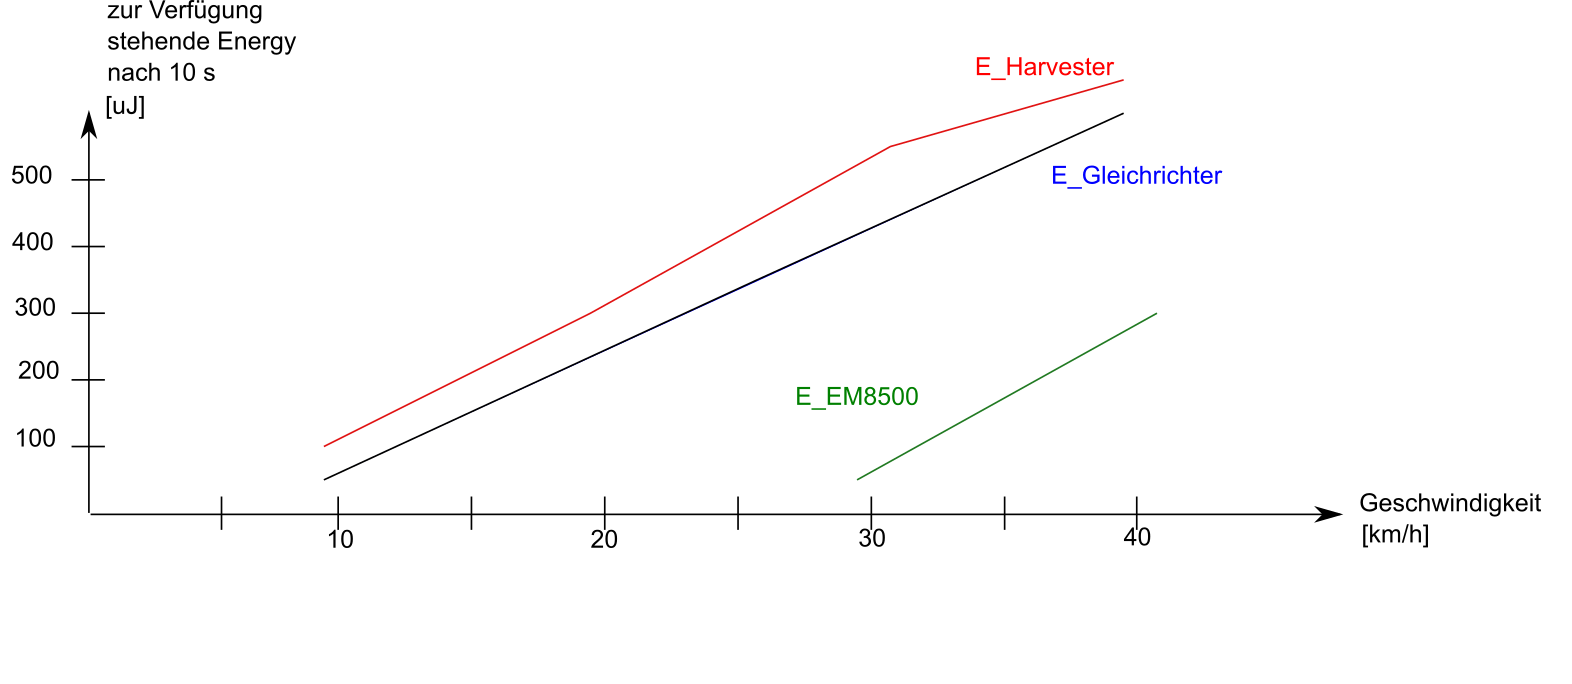
\includegraphics[width=1\textwidth]{4Resultate/imag/EnergyGewinnNachStelle.png} 
\caption{Energiegewinn Zusammengefasst nach Stelle in der Schaltung }
\end{figure}

Der Wirkungsgrad des EM8500 liegt bei 40 km\/h  bei xxx und bei 10 km\/h bei unserer Schaltung bei xxxx. 

%todo\{wirkungsgrad EM8500 berechnen}. 



\section{Energiemanagement}

%Beim Resultat spielt das Hard- und Softwaremanagment direkt ineinander, weshalb das Ergebnisse dieser zwei Aufgaben zusammen dargestellt werden.

Durch das korrekte Einstellen der Schwellwerte beim EM8500 (siehe Unterkapitel xxx) und die korrekten Ladewerte bei den Kondensatoren (siehe Unterkaptiel xxx), ist es möglich, dass sich der LTS-Kondensator bei einer Geschwindigkeit von YYY km/h lädt (siehe Abbildung xxx). Zudem entlädt sich LTS, sobald das Sensortag am Arbeiten ist (siehe Abbildung yyyy). Beim Energiemanagement ist es somit gelungen, die Schwellwerte und Kondensatorengrössen so einzustellen, dass die Funktionalitäten des EM8500-Chips voll ausgenutzt werden können.

\begin{figure}[ht]
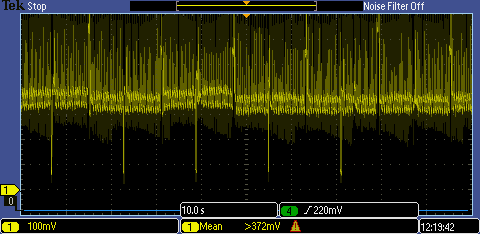
\includegraphics[width=0.1\textwidth]{4Resultate/imag/SpannungVCC.png} 
\caption{STS und LTS laden sich}
\end{figure}

\begin{figure}[ht]
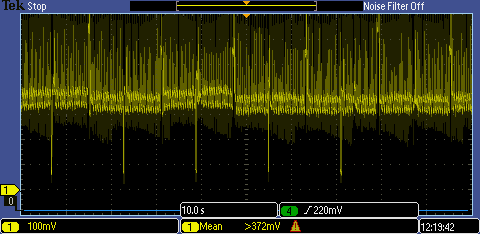
\includegraphics[width=0.1\textwidth]{4Resultate/imag/SpannungVCC.png} 
\caption{LTS liefert Energie für die Arbeitspakete}
\end{figure}


\section{Powermanagement}

Durch ein gutes Powermanagement (siehe Unterkapitel xxx) wurde es möglich, die energiestarken Aufgaben in Teilen zu erledigen. Die Abbildung xxxx zeigt, das Aufteilen der Arbeitsschritte: Zuerst folgt das Init, dann folgt das Auslesen eines Sensors, dann das Senden des Sensors. Die Aufgaben wurden aufgeteilt, weil alle drei Schritte in einem zu viel Energie verbraucht hätte, sodass VSUP zusammengebrochen wäre.

\begin{figure}[ht]
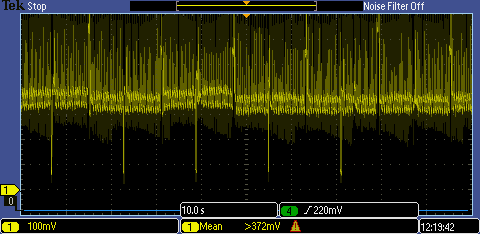
\includegraphics[width=0.1\textwidth]{4Resultate/imag/SpannungVCC.png} 
\caption{Drei Arbeitspakte bis zum Senden der Daten }
\end{figure}

%Ev.  Grossaufnahme: BLE Energieverbrauch

Die Abbildung \ref{resultat_E_Verbrauch_Verarbeitungsaufwand} zeigt den Energieverbrauch nach Verarbeitungsaufwand. Am wenigsten Energie benötigt das Berechnen der Geschwindigkeit über den RTC. Deutlich mehr Energie braucht das Auslesen der Sensor-Daten. Dies einerseits, weil die I2C-Kommunikation aufgebaut werden muss und weil die Sensoren eine gewisse Zeit brauchen, bis sie aktiv sind \todo{Aufwachzeit eines Sensors messen}. Die unterschiedlich verbrauchten Energiemengen entsprechen exakt den unterschiedlichen Startzeiten der Sensoren. 

\begin{figure}[ht]
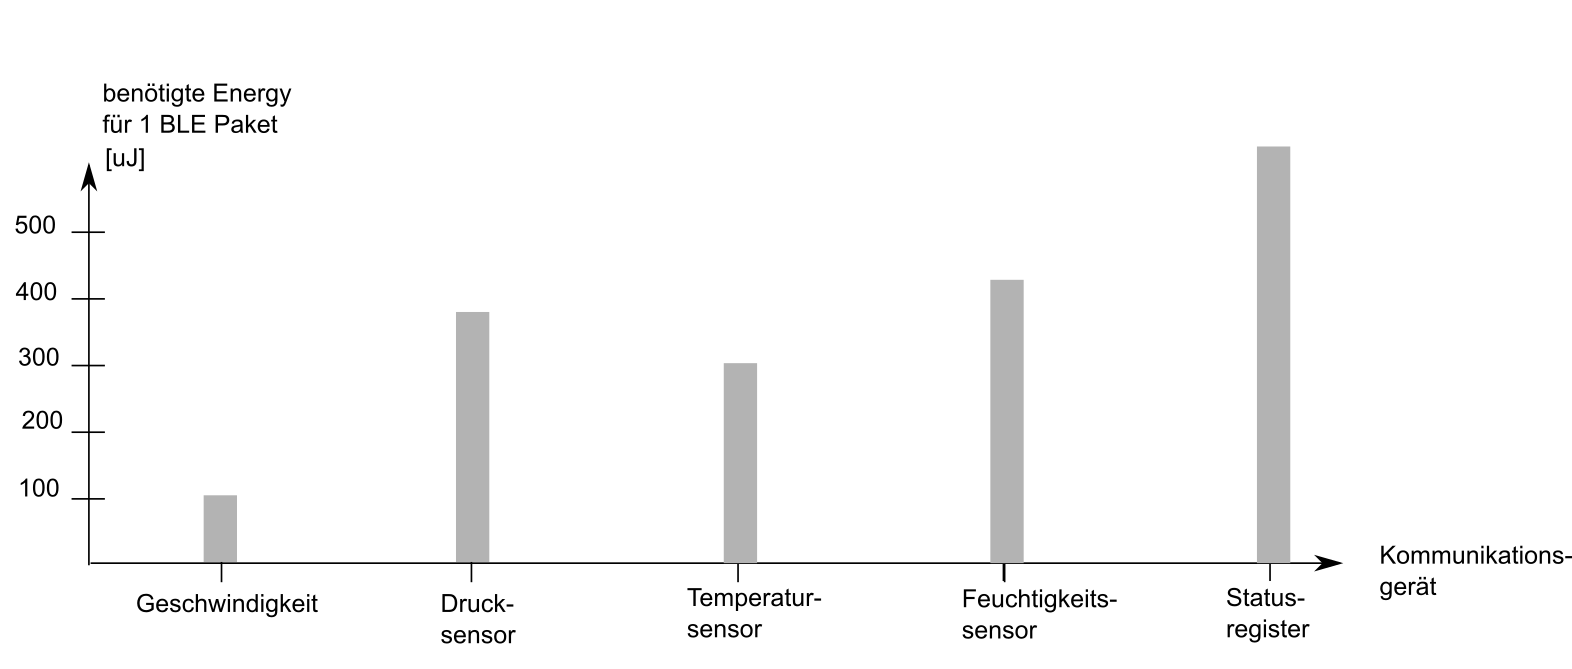
\includegraphics[width=1\textwidth]{4Resultate/imag/EnergyVerbrauchNachKommunikation.png} \label{resultat_E_Verbrauch_Verarbeitungsaufwand} 
\caption{Energieverbrauch gemäss Verarbeitungsaufwand für CPU}
\end{figure}

Kombiniert man den Energieverbrauch mit der zur Verfügung stehenden Energie am Ausgang nach dem EM8500-Chips, können (siehe Abbildung \ref{resultat_Zsm_Energy}) folgende Schlussfolgerungen gezogen werden:

\begin{enumerate}
    \item bla
    \item bla
    \item bla
    \item bla
\end{enumerate}

\begin{figure}[ht]
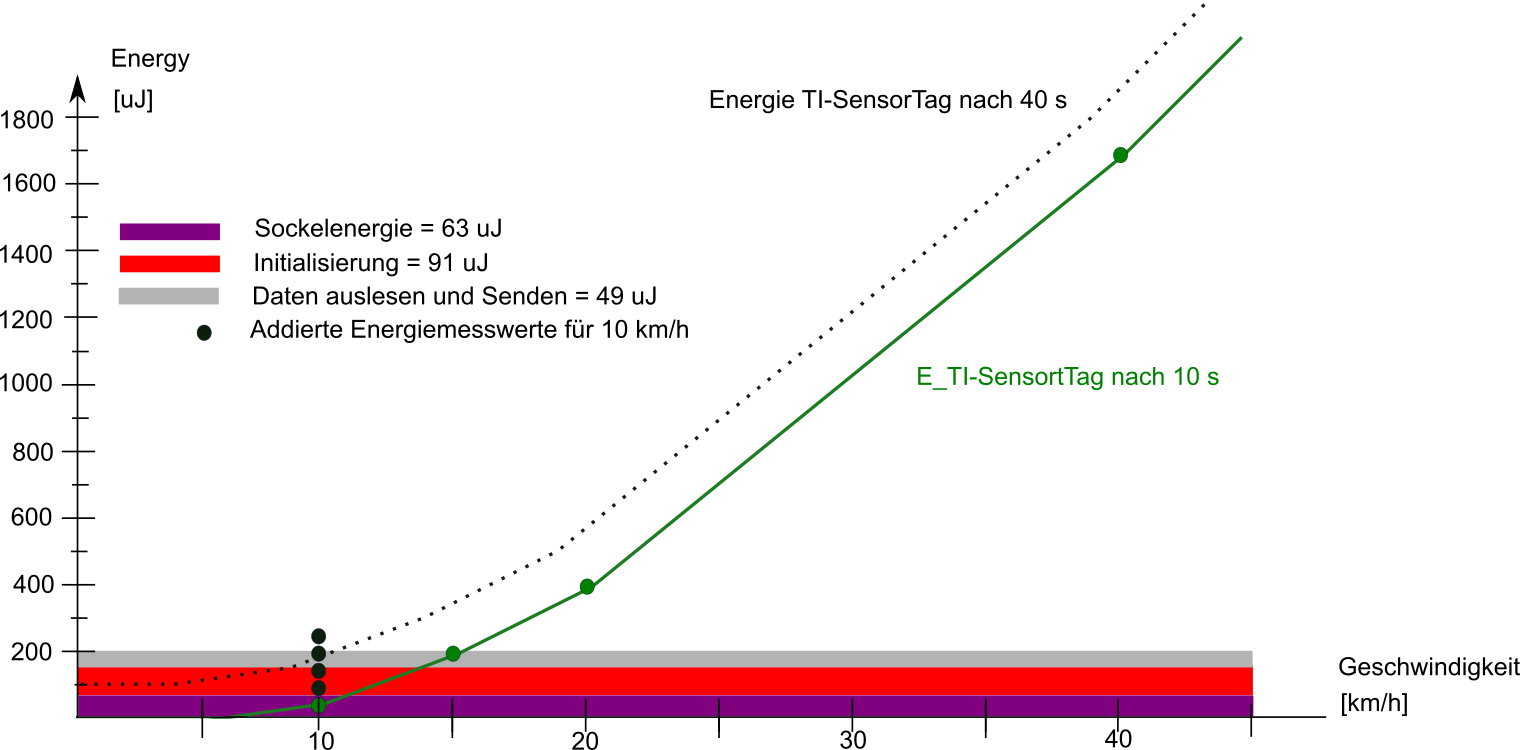
\includegraphics[width=1\textwidth]{4Resultate/imag/EnergyVerbrauchZusammenfassung.png}\label{resultat_Zsm_Energy} 
\caption{Energieverbrauch gemäss Verarbeitungsaufwand für CPU}
\end{figure}


\section{Applikation}

Bilder der App

Sniffer Screenshot

Beweis, dass Pakete ankommen

ev. Video zeiger (auf CD)






